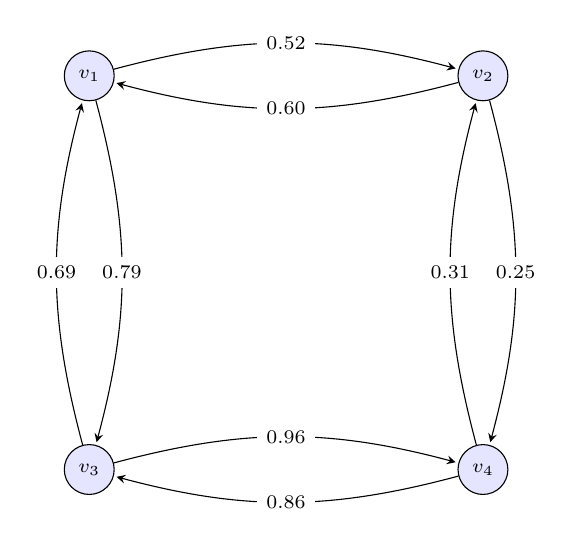
\begin{tikzpicture} [
        node distance = 5 cm, 
        font=\scriptsize, 
        vertex/.style = {circle, draw, fill=blue!10}, 
        edge/.style = {draw, -stealth, shorten >= 1pt},
        label/.style={fill=white}
    ]

    \node[vertex](1){$v_1$};
    \node[vertex, right of=1](2){$v_2$};
    \node[vertex, below of=1](3){$v_3$};
    \node[vertex, below of=2](4){$v_4$};
    
    \path[edge] (1) edge[bend left=15] node [label] {0.79} (3) edge[bend left=15] node [label] {0.52} (2);
    \path[edge] (2) edge[bend left=15] node [label] {0.25} (4) edge[bend left=15] node [label] {0.60} (1);
    \path[edge] (3) edge[bend left=15] node [label] {0.96} (4) edge[bend left=15] node [label] {0.69} (1);
    \path[edge] (4) edge[bend left=15] node [label] {0.31} (2) edge[bend left=15] node [label] {0.86} (3);;
    
\end{tikzpicture}